\begin{lemma}
The equation of  a conic with directrix $\vec{n}^{\top}\vec{x} = c$, eccentricity $e$ and focus $\vec{F}$ is given by 
\begin{align}
    \label{oct/2/30/eq:conic_quad_form}
    \vec{x}^{\top}\vec{V}\vec{x}+2\vec{u}^{\top}\vec{x}+f=0
\end{align}
where     
\begin{align}
    \label{oct/2/30/eq:conic_quad_form_v}
    \vec{V} &=\norm{\vec{n}}^2\vec{I}-e^2\vec{n}\vec{n}^{\top}, \\
    \label{oct/2/30/eq:conic_quad_form_u}
    \vec{u} &= ce^2\vec{n}-\norm{\vec{n}}^2\vec{F}, \\
    \label{oct/2/30/eq:conic_quad_form_f}
    f &= \norm{\vec{n}}^2\norm{\vec{F}}^2-c^2e^2
\end{align}
\end{lemma}
\begin{lemma}
    For $\abs{\vec{V}} \ne 0$, the length of the semi-major axis and eccentricity of the conic in \eqref{oct/2/30/eq:conic_quad_form} are given by 
    \begin{align} 
        \label{oct/2/30/eq:ab} a = \sqrt{\frac{\vec{u}^{\top}\vec{V}^{-1}\vec{u} -f}{\lambda_1}}\\
        \label{oct/2/30/eq:eccentricity} e = \sqrt{1-\frac{\lambda_1}{\lambda_2}}
    \end{align}
\end{lemma}
\begin{lemma}
Given (closest, for $\abs{\vec{V}} \neq 0$) vertex $\vec{B}$ and focus $\vec{F}$ of conic \eqref{oct/2/30/eq:conic_quad_form}, equation of directrix is given as $\vec{n}^{\top}\brak{\vec{x} - \vec{P}} = 0$ where
\begin{align}
    \vec{P} = \vec{B} + \frac{\brak{\vec{B}-\vec{F}}}{e}\\
    \vec{n} = \vec{B}-\vec{F}
\end{align}
and eccentricity
\begin{align}
    \label{oct/2/30/eq:eccentricity} e = 
    \begin{cases}
    1 & \abs{\vec{V}} = 0\\
    \dfrac{\norm{\vec{F_1}-\vec{F_2}}}{\norm{\vec{B_1}-\vec{B_2}}} & \abs{\vec{V}} \neq 0
    \end{cases}
\end{align}
\end{lemma}
\begin{proof}
For $\abs{\vec{V}}\neq 0$,

Distance between the vertices is equal to the length of the major axis. That gives,
\begin{align}
    \label{oct/2/30/eq1} \norm{\vec{B_1}-\vec{B_2}} = 2\sqrt{\frac{\vec{u}^{\top}\vec{V}^{-1}\vec{u} -f}{\lambda_1}} = 2a
\end{align}
Distance between the foci given as,
\begin{align}
    \label{oct/2/30/eq2} \norm{\vec{F_1}-\vec{F_2}} = 2\sqrt{\frac{(\vec{u}^T\vec{V}^{-1}\vec{u}-f)(\lambda_2-\lambda_1)}{\lambda_1\lambda_2}} = 2ae
\end{align}
Distance between the closest vertex and focus
\begin{multline}
    \label{oct/2/30/eq3} \norm{\vec{B}-\vec{F}} = \abs*{ \frac{\norm{\vec{B_1}-\vec{B_2}}}{2} - \frac{\norm{\vec{F_1}-\vec{F_2}}}{2}}\\
    = \abs*{\sqrt{\frac{\vec{u}^{\top}\vec{V}^{-1}\vec{u} -f}{\lambda_1}} - \sqrt{\frac{(\vec{u}^T\vec{V}^{-1}\vec{u}-f)(\lambda_2-\lambda_1)}{\lambda_1\lambda_2}}}
\end{multline}
Dividing \eqref{oct/2/30/eq1} and \eqref{oct/2/30/eq2} gives $e$

The directrix is perpendicular to the line joining vertex and focus. Thus normal vector for directrix is
\begin{align}
    \implies \vec{n} = \vec{B}-\vec{F}
\end{align}
For $\abs{\vec{V}} = 0$, the vertex is the mid-point of line joining $\vec{P}$ and $\vec{F}$
\begin{align}
    \vec{B} = \frac{\vec{P}+\vec{F}}{2}\\
    \vec{P} = 2\vec{B} + \vec{F} = \vec{B} + \frac{\brak{\vec{B}-\vec{F}}}{1}
\end{align}
$\vec{m}$ is the unit vector in the direction of $\vec{FB}$
\begin{align}
    \label{oct/2/30/unit_vec} \vec{m} = \frac{\vec{B}-\vec{F}}{\norm{\vec{B}-\vec{F}}}
\end{align}
For $\abs{\vec{V}} \ne 0$, the directrix passes through a point $\vec{P}$,
\begin{align}
    \vec{P} = \vec{B} + \vec{m}\frac{a\brak{1-e}}{e}
\end{align}
Substituting \eqref{oct/2/30/eq3}, \eqref{oct/2/30/unit_vec} gives the lemma
\end{proof}
Solution: Let the equation of the hyperbola be
\begin{align}
     \vec{x}^{\top}\vec{V}\vec{x}+2\vec{u}^{\top}\vec{x}+f=0
\end{align}
Let $\vec{B_1}, \vec{B_2}$ be the vertices and $\vec{F_1}, \vec{F_2}$ be the foci
\begin{align}
    \norm{\vec{B_1}-\vec{B_2}} = \frac{\sqrt{11}}{2}\\
    \norm{\vec{F_1}-\vec{F_2}} = 3
\end{align}
From \eqref{oct/2/30/eq:eccentricity} eccentricity,
\begin{align}
    e = \frac{\norm{\vec{F_1}-\vec{F_2}}}{\norm{\vec{B_1}-\vec{B_2}}} = \frac{6}{\sqrt{11}} 
\end{align}
Considering $\vec{B} = \myvec{0\\\frac{\sqrt{11}}{2}}, \vec{F} = \myvec{0\\3}$, the normal vector $\vec{n}$ of directrix
\begin{align}
    \vec{n} = \brak{\myvec{0\\\frac{\sqrt{11}}{2}}-\myvec{0\\3}} =  \myvec{0\\\frac{\sqrt{11}-6}{2}}
\end{align}
The directrix passes through the point $\vec{P}$,
\begin{align}
    \vec{P} = \myvec{0\\\frac{\sqrt{11}}{2}} +\frac{\sqrt{11}}{6}\brak{\myvec{0\\\frac{\sqrt{11}}{2}}-\myvec{0\\3}}= \myvec{0\\\frac{11}{12}}
\end{align}
Equation of the directrix can be given as
\begin{align}
    \myvec{0&\frac{\sqrt{11-6}}{2}}\brak{x - \myvec{0\\\frac{11}{12}}} = 0\\
    \implies \myvec{0&1}\vec{x} = \frac{11}{12}
\end{align}
Calculating $\vec{V}, \vec{u}$ and $f$,
\begin{align}
    \vec{V} &= 1^2\myvec{1&0\\0&1} - \brak{\frac{6}{\sqrt{11}}}^2\myvec{0\\1}\myvec{0&1}\\
    &= \myvec{1&0\\0&\frac{-25}{11}}
\end{align}
\begin{align}
     \vec{u} &= \frac{11}{12}\brak{\frac{6}{\sqrt{11}}}^2\myvec{0\\1} - 1^2\myvec{0\\3}=\myvec{0\\0}\\
    f &= 3^2 - \brak{\frac{11}{12}\times\frac{6}{\sqrt{11}}}^2 = \frac{25}{4}
\end{align}
Equation of the hyperbola,
\begin{align}
    \vec{x}^{\top}\myvec{1&0\\0&\frac{-25}{11}}\vec{x}+\frac{25}{4}=0
\end{align}
\begin{figure}[h]
\centering
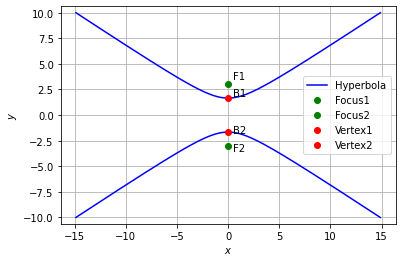
\includegraphics[width=\columnwidth]{solutions/oct/2/30/hyperbola_plot.png}
\caption{Plot of Hyperbola}
\label{oct/2/30/fig:hyperbola}
\end{figure}
